\documentclass[11pt,letterpaper]{article}
\usepackage{anysize}
\usepackage{indentfirst}
\usepackage{sectsty}
\usepackage{amsmath}
\usepackage{hyperref}
\usepackage{graphicx}
\usepackage{chngpage}
\usepackage{enumerate}
\hypersetup{
	colorlinks=true, 
	linkcolor=blue, 
	urlcolor=blue, 
	pdfnewwindow=true, 
	citecolor=black
}
\urlstyle{same}
\linespread{1.2}

\begin{document}

\begin{titlepage}
    \vspace*{4cm}
    \begin{flushright}
    {\huge
        Project 1\\[5mm]
    }
    {\large
        CS325 | Spring 2015
     }
    \end{flushright}
\hrule
    \begin{flushright}
	by Group 2\\
	Vedanth Narayanan\\
	Jonathan Merrill\\
	Tracie Lee\\
    \vfill
	\today\\
    \end{flushright}
\end{titlepage}

\raggedright

\section{Theoretical Run-time Analysis}

\subsection{Algorithm 1}
\begin{verbatim}
    maxSubarray(a[1,...,n])
        max = a[0]
        for i = [0...n]
            for j = [i,n]
                sum = 0
                for each pair(i,j) with 1<=i<=j<=n
        	        compute a[i]+a[j+1]+...+a[j-1]+a[j]
            keep max sum found so far
        return max sum found
\end{verbatim}
\textbf{Asymptotic Analysis}\\
We have $O(n^2)$ pairs * $O(n)$ time to compute each sum $= O(n^3)$.

\subsection{Algorithm 2}
\begin{verbatim}
    maxSubarray(a[1,...,n])
        for i = 1, ...., n
            sum = 0
            for = i, ...., n
                sum = sum + a[j]
                keep max sum found so far
        return max sum found
\end{verbatim}
\textbf{Asymptotic Analysis}\\
We have $O(n)$ i-iterations (outer loop) * $O(n)$ j-iterations (inner loop) * $O(n)$ for the time to update $= O(n^2)$.

\subsection{Algorithm 3}
\begin{verbatim}
    maxSubarray(a[1,...,n], initial array length)
        length = len(a)

        if length > 1:
            left = left half of array
            right = right half of array
            first = maxSubarray(left, 0)
            last = maxSubarray(right, 0)
            reverse left
            center = helper(left) + helper(right)
        else:
            first = last = center = a[0]

        if initial array length == len(a):
            PrintResults(max([first, last, center]), a, [first, last, center])

        return max([first, last, center])

    helper(a):
        max = a[0]
        sum = 0
        for i in range(0, len(a)):
            sum += a[i]
            if sum > max:
                max = sum
        return max
\end{verbatim}
\textbf{Asymptotic Analysis}\\
We have $T(n) = 2T(\frac{n}{2}) + \Theta(n)$. This falls within Case 2 of the Master Method, and therefore yields a solution of $\Theta(nlgn)$.

\subsection{Algorithm 4}
\begin{verbatim}
    maxSubarray(a[1,...,n])

    maybeStart = 0
    start = 0
    end = 0
    i = a[0]
    sum = a[0]
    small = minimum of (0, i)

    for j in range(1,len(a)):
        i = i + a[j]
        if (i - small) > sum:
            start = maybeStart
            end = j+1
            sum = (i - small)
        if i < small:
            maybeStart = j+1
            small = i
    return (sum, a, a[start:end])
\end{verbatim}
\textbf{Asymptotic Analysis}\\
We have $O(n)$ things to compute, therefore this takes $O(n)$ time.


\section{Proof of Correctness: Algorithm 3}
\subsection*{Base Case}
We pass in an array consisting of 1 element, in which case the algorithm has a check in place for an array of length greater than one, and consequently returns the same array that had been passed in since it is the max subarray within that array.

\subsection*{Inductive Hypothesis}
Assume that algorithm 3 correctly returns a maximum contiguous sum of elements $s$ from an array $A$ of $n > 1$ elements. 

\subsection*{Inductive Step}
If we split $A$ into 2 separate arrays, let $L$ represent the new array from the left side and let $R$ represent the new array from the right side. Then let $s_{i...j}$ represent any sequence of numbers with the largest sum that lies with in $S$. If the sum of $s_{i...j} = x$, then $max(first, last, center) \leq x$. There are then 3 possibilities:
\begin{enumerate}
\item $s_{i...j}$ lies completely within $L$. In this case, it would follow that the max subarray of $L$ is equal to x which means that $max(first, last, center) \geq first = x$. Because of this, we know that the answer returned is exactly x.
\item $s_{i...j}$ lies completely within $R$. In this case, it would follow that the max subarray of $R$ is equal to x which means that $max(first, last, center) \geq last = x$. Because of this, we know that the answer returned is exactly x.
\item If $s_{i...j}$ does not lie completely within $L$ or $R$, then it must start in $L$ and end in $R$. 
\end{enumerate}

\section{Testing}
\hspace{25pt}Our testing was quite thorough through out the completion of the project. The first measures taken for testing were for the correctness of our algorithms. We had written pseudo-code, and we needed to make sure that they were implemented properly. While not exactly writing unit tests, we performed manual tests. We gave the program a set list of integers, and knew what to expect as the result. The other side of our manual tests were running through the code by hand. In the beginning either we came across some indexing issues, or infinite loops, and similar issues. It was really helpful to go through by hand because it was our version of debugging, and more often than not the problems were identified and solved. In the end, we used the test cases mentioned on the project description, as well as on Canvas, and we were successfully able to pass the tests.\\
\hspace{25pt}We needed to perform some sort of "regression testing" next. This was to check the performance of our algorithms and the amount of time it took for them to run. We ended up writing a little function that generated random numbers, put them in a list, and wrote the list into the MSS\_Problems.txt file. This function still exists in our script, if it need be checked. We always wanted to write the MSS\_Problems.txt file, so we had our script accept integer values that defined the number of n's. Accordingly, we created a Makefile from where we were able to call our script with different arguments and append the results to MSS\_Results.txt. The first arguments were ones that were mentioned in the project description, but we went beyond that. For the first 2 algorithms, we found out their limits, and at that point, we decided to comment out the function calls for them, and then continue the tests for the other 2 algorithms. The last n case for Algorithm 1 was 2000. The last n case for Algorithm 2 was 30000. Both Algorithm 3 and 4 ran till n was 1000000. All this testing was done on the Flip servers, for consistent results.\\
\centerline{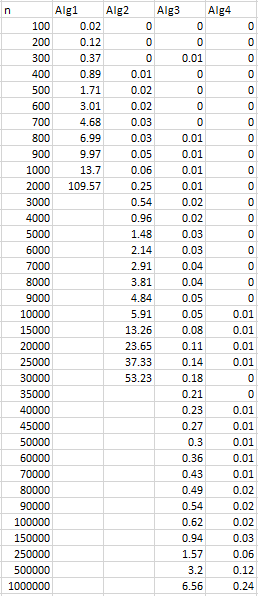
\includegraphics[width=3.5in]{TestTimes.png}}
\pagebreak

\section{Experimental Analysis}
\centerline{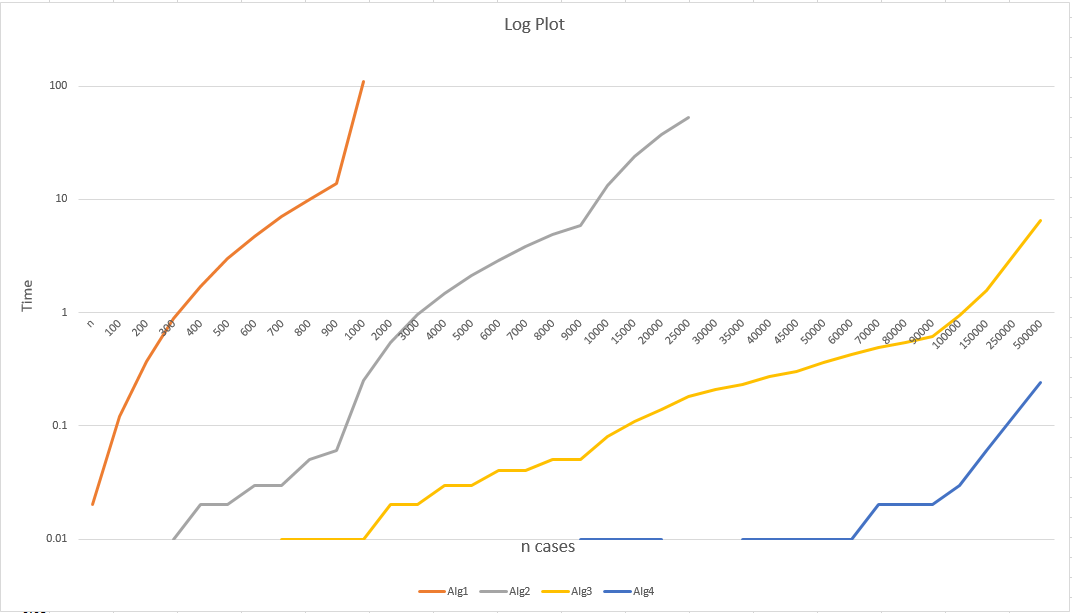
\includegraphics[width=7in]{LogPlot.png}}

\section{Extrapolation and Interpretation}
In general, our test data confirmed that our asymptotic analysis for each algorithm was very close. Algorithm was predicted to be $O(n^3)$, algorithm 2 $O(n^2)$, algorithm 3 $O(nlgn)$ and algorithm 4 $O(n)$, and all 4 algorithm plots have curves that are roughly equivalent.\vspace{8pt}
\\
To find the largest instance that can be solved within an hour for each algorithm, we had to do some rough estimating. Assuming that algorithm 1 is indeed $O(n^3)$, we used our largest testing trial for algorithm 1 ($n=2000$; completing in 109 seconds) to find the approximate number of operations the computer can do each second:\vspace{8pt}
\\
\hspace{10mm}$2000^3 / 109 = 73394495$ operations per second\vspace{8pt}
\\
Then, using the complexities we found for each algorithm, we could solve for n using a time restraint of one hour,  and the operations per second found above:\\
\begin{itemize}
\item Algorithm 1: $n=6400$
\item Algorithm 2: $n=514023$
\item Algorithm 3: $n=8.02*10^9$
\item Algorithm 4: $n=2.64*10^{11}$
\end{itemize}

\end{document}
